%!tex root = ../main.tex

\section{Background} \label{sec:background}
In this section, we introduce relevant terminology and concepts to prepare the reader for the Sections \ref{sec:research_question}--\ref{sec:implementation}.
%
We will be using many definitions from graph theory.
The Section Section \ref{sec:graphs} will introduce all needed concepts of graph theory.
%
In Section \ref{sec:distributed_computing}, we discuss about the essential concepts in the theory of distributed computing.
The section aims to explain the meaning of distributed computing and gives an introduction to the main model of distributed computing, \emph{message passing model}, from which many of the researched models inherit from.
%
In Sections \ref{sec:port_number_model} and \ref{sec:formalized_pn_model}, we introduce the port number model, and in Section \ref{sec:local_model} we introduce the LOCAL model.
These are widely used models in the field of distributed computing and they are strongly related to this work.
%
Section \ref{sec:covering_map} introduces a topological concept called \emph{covering map} that reveals a limitation of port number model.
%
We are focusing on a certain family of graph problems called \emph{Locally checkable labelling} problems.
The Sections \ref{sec:lcl_problems} and \ref{sec:lcl_problems:biregular} are dedicated to them.


\subsection{Graphs} \label{sec:graphs}
In the real world, there are many objects that are somehow related to each other.
Such things can often be visualized by a diagrams that consists of points, and lines that connect a pair of points.
A graph is a mathematical concept that abstracts the relations of these objects.
In the literature, the points are called vertices and the lines are called edges
\cite{DBLP:books/others/BondyM76}.

\begin{definition}
A graph is a tuple $$G = (V, E),$$ where $V$ is the set of vertices and $E$ is the set of edges.
%Each vertex $v \in V$
An edge $e \in E$ is a pair (2-tuple or 2-element ordered list) $e=(v, w), v, w \in V$, where vertices $v$ and $w$ are the endpoints of the edge $e$.
\end{definition}
For example, we have a graph $G=(\{1, 2, 3\}, \{(1, 2),(1, 3),(2, 3),(3, 2)\})$, and visualized it looks like the graph in Figure \ref{fig:graph1:a}.

When an edge is defined as a pair, the order of the vertices in the edge matters, that is, for all $v, w \in V, v \neq w$, we have  $(v, w) \neq (w, v)$.
We call such a graph as a \emph{directed graph} or with the shortened variation \emph{digraph}.
In an edge $(v, w)$, the first vertex $v$ points to the vertex $w$.
Usually the edge is visualized as an arrow pointing from $v$ to $w$.
One example of a directed graph is a flow graph, in which the edges represent flows from a vertex to another vertex, as seen in the Figure \ref{fig:graph1:a}.

\begin{figure}[H]
  \subcaptionbox{A simple directed graph.\label{fig:graph1:a}}%
    [.3\linewidth] {
    \centering
    \begin{tikzpicture}[>={Latex[length=3mm]},auto, on grid]
      \node[nodeSBlue] (1) {$1$};
      \node[nodeSBlue] (2) [above right = 1.3cm and 1.5cm of 1] {$2$};
      \node[nodeSBlue] (3) [below right = 1.3cm and 1.5cm of 1] {$3$};
      \draw[->] (1) edge[] node {} (2);
      \draw[->] (1) edge[] node {} (3);
      \draw[<->] (2) edge[] node {} (3);
    \end{tikzpicture}
  }
  \hfill
  \subcaptionbox{A simple undirected graph.\label{fig:graph1:b}}%
    [.3\linewidth] {
    \centering
    \begin{tikzpicture}[auto, on grid, ]
      \node[nodeSBlue] (1) {$1$};
      \node[nodeSBlue] (2) [above right = 1.3cm and 1.5cm of 1] {$2$};
      \node[nodeSBlue] (3) [below right = 1.3cm and 1.5cm of 1] {$3$};
      \draw[-] (1) edge[] node {} (2);
      \draw[-] (1) edge[] node {} (3);
      \draw[-] (2) edge[] node {} (3);
    \end{tikzpicture}
  }
  \hfill
  \subcaptionbox{An undirected multigraph.\label{fig:graph1:c}}%
    [.3\linewidth] {
    \centering
    \begin{tikzpicture}[auto, on grid, ]
      \node[nodeSBlue] (1) {$1$};
      \node[nodeSBlue] (2) [above right = 1.3cm and 1.5cm of 1] {$2$};
      \node[nodeSBlue] (3) [below right = 1.3cm and 1.5cm of 1] {$3$};
      \draw[-] (1) edge[] node {} (2);
      \draw[-] (1) edge[bend left] node {} (3);
      \draw[-] (1) edge[bend right] node {} (3);
      \draw[-] (2) edge[] node {} (3);
    \end{tikzpicture}
  }
  \caption{Examples of different graphs}
  \label{fig:graph1}
\end{figure}

\emph{Undirected graph} is a graph in which the order of the vertices in an edge does not matter.
An edge of an undirected graph is defined as an unordered pair $\{v, w\} \in E$, therefore the following holds:
\begin{equation}
\forall v, w \in V\colon \{v, w\} = \{w, v\}
\end{equation}
For example $E=\{\{1, 2\}, \{1, 2\}, \{3, 2\}, \{2, 3\}, \{1, 3\}\}=\{\{1,2\},\{1,3\},\{2,3\}\}$.
Visualization of this graph $G=(\{1,2,3\}, E)$ can be seen in the Figure \ref{fig:graph1:b}.
For the purpose of this work, we need only undirected graphs.

The definitions of graphs shown earlier do not restrict an edge to start and end in itself ($e=(v, v)$).
This kind of an edge is called a \emph{loop}.
The definitions however restricts \emph{multiple edges} (identical parallel edges).
In order to allow multiple edges, the edge set has to be defined as a \emph{multiset}.
A graph that contains multiple edges is called a \emph{multigraph}.
Depending on the author or context, multigraphs either allow or disallow loops.
In this work, we consider multigraphs to exist without loops.

A graph that has no loops or multiple edges is called a \emph{simple graph}.
Simple graphs can either be directed or undirected and it should be explicitly mentioned when defining graphs, unless the context implies it.
As we do not need directedness of edges, let us assume that further expressions of graphs are always undirected in this work.

Suppose there is an edge $e=\{v,w\}$.
We say that vertex $v$ is \emph{incident} to $e$ and $e$ is incident to $v$.
We also say that vertex $v$ is \emph{adjacent} to $w$ and vice versa.
Similarly when two edges share a vertex, we say that the edges are \emph{adjacent}.
We can also say that $w$ is a \emph{neighbour} of $v$ and vice versa.

In a graph, the degree of a vertex is the number of edges it is incident to.
We will use the notation $\deg_G(v)$ to denote the degree of vertex $v \in V$ in graph $G=(V,E)$.
In multigraphs with loops, a loop counts as 2 to a degree.

A graph that is \emph{bipartite} has exactly two disjoint sets of vertices (we call them part $A$ and part $B$), and every edge of the graph has one endpoint in vertex of $A$ and another in $B$:
\begin{align}
V &= A \cup B\\
A \cap B &= \emptyset\\
E &=\{\{a, b\} \mid a \in A, b \in B\}
\end{align}
For bipartite graphs, the sum of degrees on $A$ and $B$ are equal:
\begin{equation}
\sum_{a\in A} \deg_G(a) = \sum_{b\in B} \deg_G(b)
\end{equation}
An example of a bipartite graph can be seen in Figure \ref{fig:graph2}.

\begin{figure}[H]
\centering
% https://tex.stackexchange.com/a/499577
\begin{tikzpicture}[thick,amat/.style={matrix of nodes,nodes in empty cells,
  row sep=1em,draw,dashed,rounded corners,
  nodes={draw,solid,circle}},
  fsnode/.style={fill=strongBlue},
  ssnode/.style={fill=strongOrange}]

  \matrix[amat,nodes=fsnode,label=above:$A$] (mat1) {
  1\\
  2\\
  };

  \matrix[amat,right=2cm of mat1,nodes=ssnode,label=above:$B$] (mat2) {
  3\\
  4\\
  5\\};

  \node (1) [left = of mat1-1-1] {$\deg_G(1)=2$};
  \node (2) [left = of mat1-2-1] {$\deg_G(2)=1$};
  \node (3) [right = of mat2-1-1] {$\deg_G(3)=1$};
  \node (4) [right = of mat2-2-1] {$\deg_G(4)=1$};
  \node (5) [right = of mat2-3-1] {$\deg_G(5)=1$};
  \draw (mat1-1-1) edge (mat2-1-1);
  \draw (mat1-1-1) edge (mat2-2-1);
  %\draw (mat1-2-1) edge (mat2-2-1);
  \draw (mat1-2-1) edge (mat2-3-1);
\end{tikzpicture}
\caption{A simple disconnected bipartite graph.\label{fig:graph2}}
\end{figure}

If all vertices in a graph have the same degree, then the graph is called \emph{regular}.
For example, if every vertex in a bipartite graph shares a degree, then we call it a regular bipartite graph. When every node $a$ of part $A$ share a degree and every node $b$ of part $B$ share a degree, we call it \emph{a biregular graph}.
In fact, we use a notation $(d_A,d_B)$-biregular, where $d_A$ and $d_B$ denote the degrees of the nodes inside parts $A$ and $B$ respectively.
We can see an example of a (3,2)-biregular in Figure \ref{fig:graph3}.
The bipartite graph in Figure \ref{fig:graph2} is not biregular because the nodes in part $A$ do not share a degree i.e. for all nodes $v, w \in A$ the condition $\deg_G(v) = \deg_G(w)$ does not hold.

\begin{figure}[H]
\centering
% https://tex.stackexchange.com/a/499577
\begin{tikzpicture}[thick,amat/.style={matrix of nodes,nodes in empty cells,
  row sep=1em,draw,dashed,rounded corners,
  nodes={draw,solid,circle}},
  fsnode/.style={fill=strongBlue},
  ssnode/.style={fill=strongOrange}]

  \matrix[amat,nodes=fsnode,label=above:$A$] (mat1) {
  1\\
  2\\
  };

  \matrix[amat,right=2cm of mat1,nodes=ssnode,label=above:$B$] (mat2) {
  3\\
  4\\
  5\\};

  \node (1) [left = of mat1-1-1] {$\deg_G(1)=3$};
  \node (2) [left = of mat1-2-1] {$\deg_G(2)=3$};
  \node (3) [right = of mat2-1-1] {$\deg_G(3)=2$};
  \node (4) [right = of mat2-2-1] {$\deg_G(4)=2$};
  \node (5) [right = of mat2-3-1] {$\deg_G(5)=2$};
  \draw (mat1-1-1) edge (mat2-1-1);
  \draw (mat1-1-1) edge (mat2-2-1);
  \draw (mat1-1-1) edge (mat2-3-1);
  \draw (mat1-2-1) edge (mat2-1-1);
  \draw (mat1-2-1) edge (mat2-2-1);
  \draw (mat1-2-1) edge (mat2-3-1);
\end{tikzpicture}
\caption{A simple (3,2)-biregular graph.\label{fig:graph3}}
\end{figure}


A graph is considered as \emph{connected} if from every node one can traverse through the edges to all other nodes i.e. every pair of nodes need to also be connected.
For instance, the graph in Figure \ref{fig:graph2} has two isolated vertex subsets $\{2, 5\}$ and $\{1, 3, 4\}$, therefore the graph is \emph{disconnected}.
On the other hand, the graphs in Figures \ref{fig:graph1:b}, \ref{fig:graph1:c} and \ref{fig:graph3} are connected.
Let us not worry about the connectivity of the directed graph on Figure \ref{fig:graph1:a} as directed graphs are not relevant to this work other than in this section.

A \emph{distance} between two nodes $u, v\in V$ is the length of the shortest path between $u$ and $v$ (see Figure \ref{fig:graph4:b}).
We use the notation $\operatorname{dist}(u, v)$ for the distance between $u$ and $v$.
The maximum of all shortest paths in a graph $G$ is called the \emph{diameter} of $G$.
A \emph{subgraph} $H$ of a graph $G=(V, E)$ is a graph formed from a subset $V'$ of vertices of $V$ and a subset $E'$ of edges of $E$ such that each endpoint of $e' \in E'$ must be in $V'$.
A $r$-radius \emph{ball} of node $u$ of graph $G$ is a subgraph $H=(V', E')$ of $G$ containing:
\begin{itemize}
  \item every vertex $v\in V$ such that the distance from $u$ to $v$ is at most $r$,
  \item every edge $(u', v') \in E$ such that $u'$ and $v'$ are also in $V'$.
\end{itemize}
We use the notation $B_G(u, r)$ to denote the $r$-radius ball of node $u$ of graph $G$.
For an example of a ball, see the Figure \ref{fig:graph5}.

\begin{figure}[H]
  \subcaptionbox{A path between nodes 1 and 5 in a graph $G$.
  The length of the path is 4.
  \label{fig:graph4:a}}
    [.30\linewidth] {
    \centering
    \begin{tikzpicture}[]
      \node[nodeSBlue] (1) [] at (0,0) {$1$};
      \node[nodeSBlue] (2) [right =  of 1] {$2$};
      \node[nodeSBlue] (3) [right =  of 2] {$3$};
      \node[nodeSBlue] (4) [below =  of 1] {$4$};
      \node[nodeSBlue] (5) [below =  of 2] {$5$};
      \node[nodeSBlue] (6) [below =  of 3] {$6$};
      \node[nodeSBlue] (7) [below =  of 4] {$7$};
      \node[nodeSBlue] (8) [below =  of 5] {$8$};
      \node[nodeSBlue] (9) [below =  of 6] {$9$};
      \draw[highlight] (1) -- (2);
      \draw[highlight] (2) -- (3);
      \draw[] (4) -- (5);
      \draw[highlight] (5) -- (6);
      \draw[] (1) -- (4);
      \draw[] (2) -- (5);
      \draw[highlight] (3) -- (6);
      \draw[] (4) -- (7);
      \draw[] (5) -- (8);
      \draw[] (6) -- (9);
      \draw[] (7) -- (8);
      \draw[] (8) -- (9);
    \end{tikzpicture}
  }
  \hfill
  \subcaptionbox{A shortest path between nodes 1 and 5 in a graph $G$.
  The length of the path is 2, thus $\operatorname{dist}(u,v)=2$.
  \label{fig:graph4:b}}
    [.30\linewidth] {
    \centering
    \begin{tikzpicture}[]
      \node[nodeSBlue] (1) [] at (0,0) {$1$};
      \node[nodeSBlue] (2) [right =  of 1] {$2$};
      \node[nodeSBlue] (3) [right =  of 2] {$3$};
      \node[nodeSBlue] (4) [below =  of 1] {$4$};
      \node[nodeSBlue] (5) [below =  of 2] {$5$};
      \node[nodeSBlue] (6) [below =  of 3] {$6$};
      \node[nodeSBlue] (7) [below =  of 4] {$7$};
      \node[nodeSBlue] (8) [below =  of 5] {$8$};
      \node[nodeSBlue] (9) [below =  of 6] {$9$};
      \draw[highlight={green}] (1) -- (2);
      \draw[] (2) -- (3);
      \draw[] (4) -- (5);
      \draw[] (5) -- (6);
      \draw[] (1) -- (4);
      \draw[highlight={green}] (2) -- (5);
      \draw[] (3) -- (6);
      \draw[] (4) -- (7);
      \draw[] (5) -- (8);
      \draw[] (6) -- (9);
      \draw[] (7) -- (8);
      \draw[] (8) -- (9);
    \end{tikzpicture}
  }
  \hfill
  \subcaptionbox{A path between nodes 1 and 9 illustrating the diameter of the graph $G$.
  The length of the path is 4, thus $\operatorname{diameter}(G)=4$.
  \label{fig:graph4:c}}
    [.30\linewidth] {
    \centering
    \begin{tikzpicture}[]
      \node[nodeSBlue] (1) [] at (0,0) {$1$};
      \node[nodeSBlue] (2) [right =  of 1] {$2$};
      \node[nodeSBlue] (3) [right =  of 2] {$3$};
      \node[nodeSBlue] (4) [below =  of 1] {$4$};
      \node[nodeSBlue] (5) [below =  of 2] {$5$};
      \node[nodeSBlue] (6) [below =  of 3] {$6$};
      \node[nodeSBlue] (7) [below =  of 4] {$7$};
      \node[nodeSBlue] (8) [below =  of 5] {$8$};
      \node[nodeSBlue] (9) [below =  of 6] {$9$};
      \draw[] (1) -- (2);
      \draw[] (2) -- (3);
      \draw[] (4) -- (5);
      \draw[] (5) -- (6);
      \draw[highlight={blue}] (1) -- (4);
      \draw[] (2) -- (5);
      \draw[] (3) -- (6);
      \draw[highlight={blue}] (4) -- (7);
      \draw[] (5) -- (8);
      \draw[] (6) -- (9);
      \draw[highlight={blue}] (7) -- (8);
      \draw[highlight={blue}] (8) -- (9);
    \end{tikzpicture}
  }
  \caption{Examples of different kind of paths illustrated by highlighting the edges that form the path.}
  \label{fig:graph4}
\end{figure}

\begin{figure}[H]
  \subcaptionbox{The graph $G$ from Figure \ref{fig:graph4}.
  Inside the red area is each node with distance at most 1 to node 5.
  \label{fig:graph5:a}}
    [.45\linewidth] {
    \begin{tikzpicture}[]
      \node[nodeSBlue] (1) [] at (0,0) {$1$};
      \node[nodeSBlue] (2) [right =  of 1] {$2$};
      \node[nodeSBlue] (3) [right =  of 2] {$3$};
      \node[nodeSBlue] (4) [below =  of 1] {$4$};
      \node[nodeSBlue] (5) [below =  of 2] {$5$};
      \node[nodeSBlue] (6) [below =  of 3] {$6$};
      \node[nodeSBlue] (7) [below =  of 4] {$7$};
      \node[nodeSBlue] (8) [below =  of 5] {$8$};
      \node[nodeSBlue] (9) [below =  of 6] {$9$};
      \draw[] (1) -- (2);
      \draw[] (2) -- (3);
      \draw[] (4) -- (5);
      \draw[] (5) -- (6);
      \draw[] (1) -- (4);
      \draw[] (2) -- (5);
      \draw[] (3) -- (6);
      \draw[] (4) -- (7);
      \draw[] (5) -- (8);
      \draw[] (6) -- (9);
      \draw[] (7) -- (8);
      \draw[] (8) -- (9);
      \draw[red] \convexpath{4,2,6,8}{0.5cm};
    \end{tikzpicture}
    }
    \hfill
    \subcaptionbox{A 1-radius ball $B_G(5, 1)$ is a subgraph of $G$.
    \label{fig:graph5:b}}
      [.45\linewidth] {
      \begin{tikzpicture}[]
        \node[draw=none, minimum size=0.7cm] (1) [] at (0,0) {};
        \node[nodeSBlue] (2) [right =  of 1] {$2$};
        \node[draw=none, minimum size=0.7cm] (3) [right =  of 2] {};
        \node[nodeSBlue] (4) [below =  of 1] {$4$};
        \node[nodeSBlue] (5) [below =  of 2] {$5$};
        \node[nodeSBlue] (6) [below =  of 3] {$6$};
        \node[draw=none, minimum size=0.7cm] (7) [below =  of 4] {};
        \node[nodeSBlue] (8) [below =  of 5] {$8$};
        \node[draw=none, minimum size=0.7cm] (9) [below =  of 6] {};
        %\draw[] (1) -- (2);
        %\draw[] (2) -- (3);
        \draw[] (4) -- (5);
        \draw[] (5) -- (6);
        %\draw[] (1) -- (4);
        \draw[] (2) -- (5);
        %\draw[] (3) -- (6);
        %\draw[] (4) -- (7);
        \draw[] (5) -- (8);
        %\draw[] (6) -- (9);
        %\draw[] (7) -- (8);
        %\draw[] (8) -- (9);
        %\draw[red] \convexpath{4,2,6,8}{0.5cm};
      \end{tikzpicture}
      }
  \caption{Example of a ball.}
  \label{fig:graph5}
\end{figure}


\subsection{Distributed computing} \label{sec:distributed_computing}
Executing a computer program in several identical or different computers is called distributed computing
\cite{DBLP:books/el/leeuwen90/LamportL90}.
It is similar to running a computer program that contains multiple concurrent tasks, in a computer, but in distributed computing there are higher level tasks that are distributed to different computer nodes.

Computers are called nodes, and they are connected to each other with communication channels.
These communication channels carry data from a node to another node.
Together, nodes and communication channels form a network.
A common way to visualize these networks is by drawing a graph in which the nodes represent computing nodes and edges represent the communication channels.
\cite{HirvonenSuomelaDistAlg2020}


\begin{figure}[H]
  \subcaptionbox{A small distributed network containing 5 nodes.
    \label{fig:dist_comp1:a}
  }%
    [.45\linewidth] {
    \centering
  \begin{tikzpicture}[every node/.style={circle,thick,draw}]
    \node[nodeSBlue] (1) {};
    \node[nodeSBlue] (2) [ right of=1] {};
    \node[nodeSBlue] (3) [ right of=2] {};
    \node[nodeSBlue] (4) [ right of=3] {};
    \node[nodeSBlue] (5) [ right of=4] {};
    \draw (1) -- (2);
    \draw (2) -- (3);
    \draw (3) -- (4);
    \draw (4) -- (5);
  \end{tikzpicture}
  }
  \hfill
  \subcaptionbox{
    A larger distributed network containing 120 nodes.
    \label{fig:dist_comp1:b}
  }%
    [.45\linewidth] {
    \centering
  \resizebox{0.45\textwidth}{!}{%
  \begin{tikzpicture}[every node/.style={circle,thick,draw}]
    \pgfmathtruncatemacro{\maxX}{14}
    \pgfmathtruncatemacro{\maxY}{7}
    \pgfmathtruncatemacro{\maxXm}{\maxX - 1}
    \pgfmathtruncatemacro{\maxYm}{\maxY - 1}
    % Nodes
    \foreach \x in {0,...,\maxX}
      \foreach \y in {0,...,\maxY}
           \node [nodeSBlue]  (\x\y) at (\x,\y) {};
    % Vertical edges
    \foreach \x [count=\xi] in {0,...,\maxX}
      \foreach \y [count=\yi] in {0,...,\maxYm} {
        \draw (\x\y)--(\x\yi);
      }
    % Horizontal edges
    \foreach \x [count=\xi] in {0,...,\maxXm}
      \foreach \y [count=\yi] in {0,...,\maxY} {
        \draw (\x\y)--(\xi\y);
      }
  \end{tikzpicture}
  }%
%    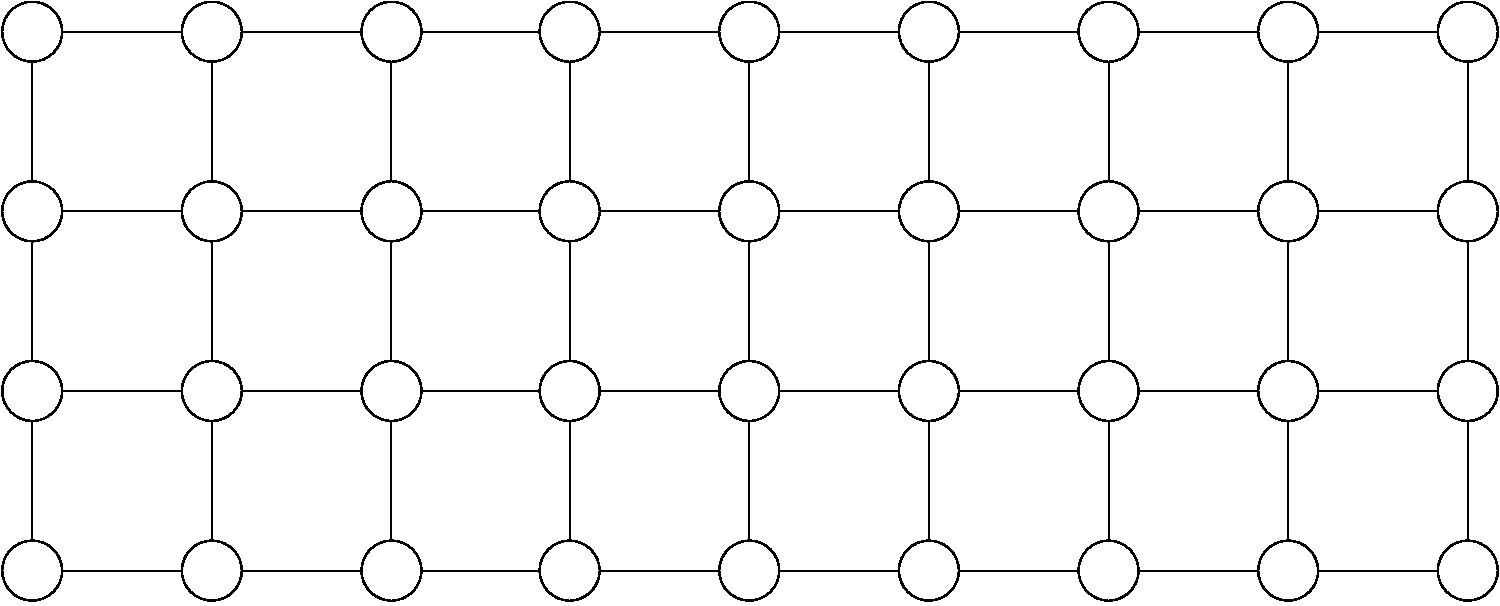
\includegraphics[scale=0.4]{diagrams/dist_comp1.pdf}
    %\missingfigure{A bigger distributed network example}
  }
  \caption{Examples of distributed networks.}
  \label{fig:dist_comp1}
\end{figure}
According to Lamport \cite{DBLP:books/el/leeuwen90/LamportL90}, in the area of distributed computing, the term \emph{model} denotes a view or abstract representation of a distributed system.
There are multiple different computation models used in distributed computing \cite{DBLP:books/el/leeuwen90/LamportL90}.
The most important category of distributed computation models is \emph{process models} \cite{DBLP:books/el/leeuwen90/LamportL90}.
In process models, the work or activities are represented as concurrently executed processes that execute their instructions sequentially \cite{DBLP:books/el/leeuwen90/LamportL90}.
A standard way to distinguish different process models from each other is to categorise them by the method they use to communicate with each other (\emph{interprocess communication}) \cite{DBLP:books/el/leeuwen90/LamportL90}.


%\subsubsection{Message passing model} \label{sec:message_passing_model}
Message passing models are one form of a process model \cite{DBLP:books/el/leeuwen90/LamportL90}.
In the model, processes communicate by adding a message to a message queue, and the recipient process moves the message out (dequeues) from the message queue \cite{DBLP:books/el/leeuwen90/LamportL90}.

Different message passing models are widely used in the research field of distributed computing.
The models can vary in different details, such as in the size of the message queues \cite{DBLP:books/el/leeuwen90/LamportL90}, in the size of the messages \cite{peleg2000distributed} and on how the nodes get identified \cite{DBLP:conf/focs/Linial87}, if they are identified at all \cite{DBLP:conf/istcs/MayerNS95}.
%As the message passing models itself can be defined in multiple ways \cite{DBLP:books/el/leeuwen90/LamportL90}, we will use a definition from which the relevant models commonly inherit from.
We will dive deeper into the most relevant message passing models for this work in Sections \ref{sec:port_number_model} and \ref{sec:local_model}.

An algorithm that is executed in a distributed fashion in a distributed network, is called as a distributed algorithm.
Each node in a network is started simultaneously and will always execute the same algorithm.
Initially the nodes are on the same state and there can be finitely or infinitely many states.
Initially the nodes are aware of only themselves and of the connections to their neighbours.
One might question that if every node starts with the same state, would not they also end up in the same state?
Well yes, this happens inevitably in a case where the nodes were not given any additional symmetry breaking inputs and if every node sees the same amount of neighbours \cite{HirvonenSuomelaDistAlg2020}.

%For example, we have a chain like network $W$ where each node $w$ has exactly two neighbours.
%The task is to execute an algorithm that finds the number of nodes in the network.


In practice, every computer node on a network has an UUID (Universally unique identifier) that can be used to break the symmetry, and nodes are usually given some input data that they process, and nodes can always randomize data as they are never completely synchronized together, so this is not necessarily a problem.
In theory, we explicitly have to assume that there exists these kind of symmetry breaking elements.
In this works, distributed algorithms are deterministic unless otherwise mentioned.
In other research there might be randomizing involved.


%TODO Find a correct place to talk  about execution times if there is any}
%In the message passing model, one could easily think that the execution time of the algorithm is the standard unit used to measure the performance but this is not true.
%The message passing model implies that the dominant cost during an execution of a distributed algorithm is the message passing itself
%\cite{DBLP:books/el/leeuwen90/LamportL90}.
%This really...
%TODO continue here




%The following two sections (\ref{sec:port_number_model} and \ref{sec:local_model} ) talk about different forms of message passing models that are highly relative to this paper.

\subsection{Port number model} \label{sec:port_number_model}
This section is based on the excellent textbook \cite{HirvonenSuomelaDistAlg2020} unless otherwise mentioned.

Port number model (PN model) is a rather weak model of computation that inherits from the message passing model.
In the model, nodes do not have identification.
A distributed algorithm that executes in a port number model is called as a PN-algorithm.

%We can basically take any network $N$ that has the same structure as a simple undirected graph $G$.
%Each vertex of $G$ can be one-to-one mapped (bijection) to the nodes of $N$ and vice-versa.
%Respectively all edges $(v, w)$ of $G$ can be mapped to communication channels between nodes $v$ and $w$.

Communication channels start and end from communication ports.
Each node has communication ports numbered from $1$ to $d$, where $d$ is the degree of the node.
The ports are numbered in an arbitrary order.

All nodes are considered identical; initially they are in the same internal state.
Every node starts the execution simultaneously following the same PN-algorithm $A$.
The execution of $A$ is done synchronously in parallel.
A communication round consists of following synchronous steps:
\begin{enumerate}
  \item send a message to each port,
  \item wait until all messages have been sent,
  \item receive a message from each port,
  \item update internal state.
\end{enumerate}
After each communication round, a node can optionally stop execution and announce its local output.
All nodes are required to eventually stop.
When all nodes have stopped, the algorithm is considered as stopped.
The running time of the algorithm $A$ is the total communication rounds that took place.


\subsection{Formalized port number model} \label{sec:formalized_pn_model}
In Section \ref{sec:port_number_model} we briefly and informally introduced the PN model.
Now in this section and in the following subsections we give a more formal definition to the PN model.
As in the previous section, this section is based on the textbook \cite{HirvonenSuomelaDistAlg2020} unless otherwise mentioned.

PN network is a 3-element tuple $N = (V, P, p)$, where $V$ and $P$ are the sets of vertices and ports respectively, and $p\colon P \rightarrow P$ is a function that maps a port to another port, forming a communication channel.
A port, an element of $P$, is a pair $(v, i)$ where $v \in V$ and $i \in \{1, 2, \dotsc\}$.
Additionally we assume that $p$ is an involution, that is, for all ports $x \in P$ we have $p(p(x)) = x, $ i.e. each edge of the ``underlying graph'' is undirected.
See Figures \ref{fig:formal_pn1:a} and \ref{fig:formal_pn1:b} for examples of valid and invalid PN networks.

\begin{figure}[H]
  \subcaptionbox{A PN network of two nodes, $a$ and $b$.
    Both $a$ and $b$ have degree of 2, therefore 2 ports.
    Ports are $(a, 1), (a, 2), (b, 1)$ and $(b, 2)$.
    The connections are
      $p((a, 1)) = (b, 1)$,
      $p((a, 2)) = (b, 2)$,
      $p((b, 1)) = (a, 1)$ and
      $p((b, 2)) = (a, 2)$.
    \label{fig:formal_pn1:a}
  }%
    [.45\linewidth] {
    \centering
    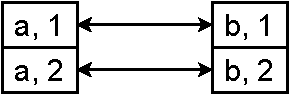
\includegraphics[scale=0.6]{diagrams/formalizing_pn_network_diagram1.pdf}
  }
  \hfill
  \subcaptionbox{
    An invalid PN network as port mapping function $p$ is not an involution:
    $p(p((a, 1))) = p(p((a, 2))) \neq (a, 1)$.
    \label{fig:formal_pn1:b}
  }%
    [.45\linewidth] {
    \centering
    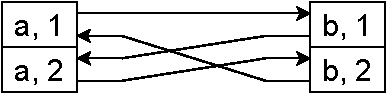
\includegraphics[scale=0.6]{diagrams/formalizing_pn_network_diagram2.pdf}
  }
  \caption{Examples of a valid and an invalid PN network.}
  \label{fig:formal_pn1}
\end{figure}


The degree $\deg_N(v)$ of a node $v \in V$ is equal to the number of ports of $v$.
We assume that the port numbers are consecutive positive integers starting from 1, i.e. the ports of a node $v$ are $\{(v, i) \mid i \in \{1, 2, \dotsc, \deg_N(v)\}\}$.
Note that the highest port number of $v$ is also the degree of $v$.

When we say \emph{port number $i$ in node $v$}, we refer to the port $(v, i)$.
When we say \emph{port $(v, i)$ is connected to port $(w, j)$}, we refer to $p((v, i)) = (w, j)$.

A loop is a connection where port $(v, i)$ is connected to port $(v, j)$.
For example there are two loops, $p((a, 1)) = (a, 2)$ and $p((c,2)) = (c,2)$, in Figure \ref{fig:formal_pn2:c}.

There are multiple connections between two distinct nodes $v$ and $w$ if $p((v, i_1)) = (w, j_1)$, $p((v, i_2)) = (w, j_2)$, $i_1 \neq j_1$ and $i_2 \neq j_2$.
For example there are connections $p((b, 2)) = (d, 1)$ and $p((b, 3)) = (d, 2)$ in Figure \ref{fig:formal_pn2:c}.

If a PN network has neither loops or multiple connections, it is called a \emph{simple} PN network.
For example the network is simple in Figure \ref{fig:formal_pn2:a}.


\begin{figure}[H]
  \subcaptionbox{
    A simple PN network.
    The underlying graph is also simple.
    \label{fig:formal_pn2:a}
  }%
    [.3\linewidth] {
    \centering
    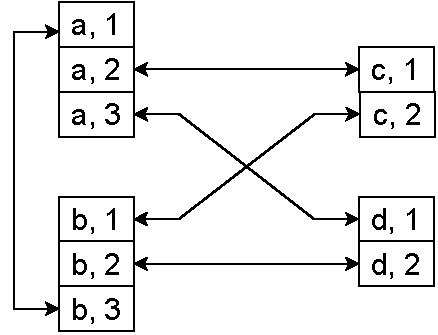
\includegraphics[scale=0.55]{diagrams/formalizing_pn_network_diagram4.pdf}
  }
  \hfill
  \subcaptionbox{
    An alternative representation of the PN network from Figure \ref{fig:formal_pn2:b}
    \label{fig:formal_pn2:b}
  }%
    [.3\linewidth] {
    \centering
    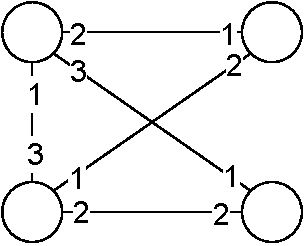
\includegraphics[width=0.3\textwidth]{diagrams/formalizing_pn_network_diagram5.pdf}
  }
  \hfill
  \subcaptionbox{
    A PN network with loops and parallel connections.
    This kind of network cannot be shown in the alternative representation unlike the network on Figure \ref{fig:formal_pn2:a}.
    \label{fig:formal_pn2:c}
  }%
    [.3\linewidth] {
    \centering
    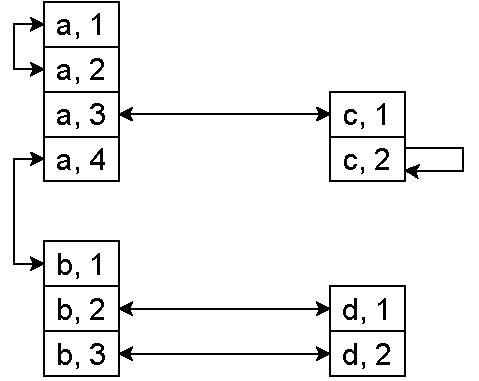
\includegraphics[scale=0.55]{diagrams/formalizing_pn_network_diagram3.pdf}
  }
  \caption{Examples of simple and non simple PN networks.}
  \label{fig:formal_pn2}
\end{figure}


\subsubsection{Underlying graph} \label{sec:underlying_graph}

Each simple PN network $N=(V,P,p)$ has an \emph{underlying graph} $G=(V,E)$.
An edge $\{v, w\}$ is part of the underlying network $G$ if and only if $v$ is connected to $w$, that is, $E = \{ \{v, w\} \mid  p((v, i)) = (w, j) \}$.
A network with multiple connections uses the same definition to determine an underlying network, but in that case $E$ has to be a multiset instead of a set, in order to allow multiple same edges.

In case an underlying graph of a network is connected, we say that \emph{the network is connected.}
Throughout this work, we assume that the introduced networks are connected.

\begin{figure}[H]
  \subcaptionbox{
    An underlying simple graph of the simple PN network from Figure \ref{fig:formal_pn2:a} and Figure \ref{fig:formal_pn2:b}.
    \label{fig:underlying_graphs1:a}
  }%
    [.45\linewidth] {
    \centering
    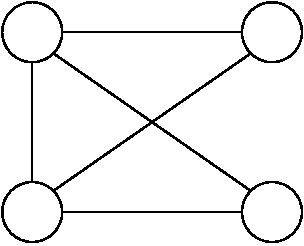
\includegraphics[scale=0.6]{diagrams/formalizing_pn_network_underlying_graph_1.pdf}
  }
  \hfill
  \subcaptionbox{
    An underlying multigraph of the PN network with multiple connections in Figure \ref{fig:formal_pn1:a}.
    \label{fig:underlying_graphs1:b}
  }%
    [.45\linewidth] {
    \centering
    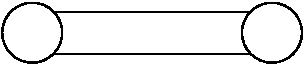
\includegraphics[width=0.3\textwidth]{diagrams/formalizing_pn_network_underlying_graph_2.pdf}
  }
  \caption{Examples of underlying graphs.}
  \label{fig:underlying_graphs1}
\end{figure}

%\subsubsection{Node labelings}
\subsubsection{Distributed graph problems} \label{sec:dist_graph_probl}
Researchers are often interested in different distributed graph problems.
These problems always have some kind of set of solution.
As it turns out, many of these problems can be encoded using the node labelings.

%TODO feels like this needs a smooth transition from the previous topic
Node labelings are a way to associate information with each node $v \in V$.
It is defined as a function $f\colon V \rightarrow Y$, where $Y$ is an arbitrary set of labels.

We can use the concept of node labelings to represent subsets $X_1, X_2, \dotsc, X_n \in V$ for some $n \in \mathbb{Z}_{>0}$ with node labeling $g\colon V \rightarrow \{1, 2, \dotsc, n\}$ where $g(v) = i$ indicates that $v \in X_i$ and $v \notin X_j, j \neq i$.
Note that the subsets $X_1, X_2, \dotsc, X_n$  are disjoint, and $X_1 \cup X_2 \cup \dotsb \cup X_n = V$.

Let $\Pi$ be a distributed graph problem.
The value of $\Pi(N)$ is the set of solutions, where $N=(V, P, p)$ is a simple PN network.
A solution $f \in \Pi(N)$ is a node labeling $f\colon V \rightarrow Y$, where $Y$ is some set of local outputs specific to the problem in question.

%Next we will give some examples of distributed graph problems and what kind of node labelings their solutions have.
For example:
\begin{description}
  \item[Vertex cover] of a graph $G$ is a subset $V' \subseteq V$ of nodes which together \emph{cover} all edges of the graph, that is, at least one endpoint from each edge must be in the subset $V'$.
  A node labeling $f$ is a solution $f \in \Pi(N)$ if $f$ encodes a vertex cover of the underlying graph $G$ of $N$.
  \item[Independent set] of a graph $G$ is a subset $V' \subseteq V$ of nodes where no two nodes are adjacent. That is, for each $u, v, \in V' s.t. u \neq v$, an edge $(u, v)$ is not in $E$.
  A node labeling $f$ is a solution $f \in \Pi(N)$ if $f$ encodes an independent set of nodes of the underlying graph $G$ of $N$.
  \item[Maximal independent set] of a graph $G$ is an independent subset $V' \subseteq V$ of nodes such that there is no additional vertex $w \in V \backslash V'$ that can be included in $V'$ such that it stays as an independent set.
  A node labeling $f$ is a solution $f \in \Pi(N)$ if $f$ encodes an independent set of nodes of the underlying graph $G$ of $N$.
  \item[$k$-coloring] of a graph $G$ is partition of $V$ with $k$ subsets $X_1, X_2, \dotsc, X_k$ where each subset is an independent set.
  A node labeling $f$ is a solution $f \in \Pi(N)$ if $f$ encodes a $k$-coloring of the underlying graph $G$ of $N$.
\end{description}

In the first three problems it seems like we are looking for only one subset of vertices $V' \subseteq V$.
Indeed, but we also have the subset of vertices $V \backslash V'$, thus $n=2$.
Therefore we can define $X_1 = V'$ and $X_2 = V \backslash V'$.
In the problem $k$-coloring, we are looking for $k$ subsets of vertices $X_1, X_2, \dotsc, X_k$, therefore $n=k$.

\begin{figure}[H]
  \subcaptionbox{
    A vertex cover.
    \label{fig:distributed_graph_problems1:a}
  }%
    [.30\linewidth] {
    \centering
    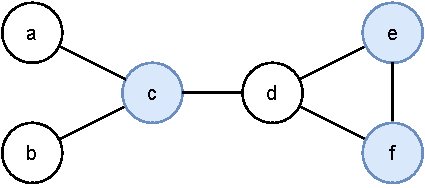
\includegraphics[width=0.30\textwidth]{diagrams/formalizing_pn_network_6.pdf}
  }
  \hfill
  \subcaptionbox{
    A maximal independent set.
    \label{fig:distributed_graph_problems1:b}
  }%
    [.30\linewidth] {
    \centering
    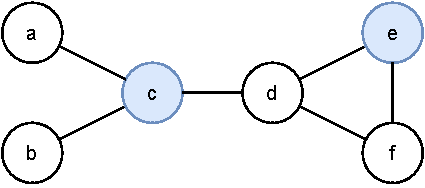
\includegraphics[width=0.30\textwidth]{diagrams/formalizing_pn_network_7.pdf}
  }
  \hfill
  \subcaptionbox{
    A 3-coloring.
    \label{fig:distributed_graph_problems1:c}
  }%
    [.30\linewidth] {
    \centering
    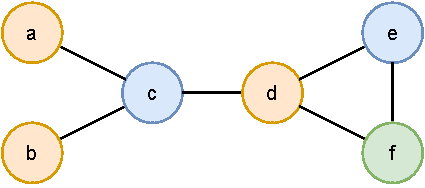
\includegraphics[width=0.30\textwidth]{diagrams/formalizing_pn_network_8.pdf}
  }
  \caption{Example solutions to different graph problems.
  In Figures \ref{fig:distributed_graph_problems1:a} and \ref{fig:distributed_graph_problems1:b}, the blue nodes form a node labeling that denote a solution.
  In Figure \ref{fig:distributed_graph_problems1:c} there are two additional labels, yellow and green in order there to be 3 labels for 3 colors.
  }
  \label{fig:distributed_graph_problems1}
\end{figure}

In Figure \ref{fig:distributed_graph_problems1} we can see two examples of graph problem encodings.
The node labeling in Figure \ref{fig:distributed_graph_problems1:a} is a vertex cover.
However, the node labeling in Figure \ref{fig:distributed_graph_problems1:b} is not a vertex cover, because there is an edge $(d, f)$ and neither of the nodes are in the solution set $\{c, e\}$.
The node labeling in Figure \ref{fig:distributed_graph_problems1:b} is a maximal independent set.
On the other hand, the node labeling in Figure \ref{fig:distributed_graph_problems1:a} is not an independent set, because there is an edge $(e, f)$ and both $e$ and $f$ are in the solution set.



\subsubsection{Distributed algorithms in the PN model}

\newcommand{\algin}{\operatorname{Input}}
\newcommand{\algstates}{\operatorname{States}}
\newcommand{\algout}{\operatorname{Output}}
\newcommand{\algmsg}{\operatorname{Msg}}

\newcommand{\alginit}{\operatorname{init}}
\newcommand{\algsend}{\operatorname{send}}
\newcommand{\algrecv}{\operatorname{receive}}

A \emph{distributed algorithm} $A$ can be described as a state machine.
The algorithm $A$ can possibly have infinitely many states or only finitely many states.
The components of $A$ are:
\begin{enumerate}
  \item $\algin_A$ is the set of local inputs,
  \item $\algstates_A$ is the set of states,
  \item $\algout_A \subseteq \algstates_A$ is the set of states that are considered as output states,
  \item $\algmsg_A$ is the set of messages.
\end{enumerate}

The algorithm always consists of 3 functions, each defined for each degree $d \in \mathbb{N}$.
The first function, $$\alginit_{A,d}\colon \algin_A \rightarrow \algstates_A$$ initializes the state of the calling node using the given input data.
%The degree $d$ is also parameterized into the function meaning that the function can operate differently with different degree nodes.
Each node calls the function $\alginit_{A,d}$ as its first function call.

After initialization, each node constructs messages for each of their neighbour by calling the second function:
$$\algsend_{A,d}\colon \algstates_A \rightarrow \algmsg_A^d$$
A node gives its current local state as an input to the function and the returning value is a $d$-element tuple of messages.

The third function allows nodes to receive messages from each of their neighbours.
It is defined as:
$$\algrecv_{A,d}\colon \algstates_A \times \algmsg_A^d \rightarrow \algstates_A$$
The function is given a node's current state and a $d$-element tuple of received messages.
In return, it gives a state value that represents the node's new state.
Additionally whenever the current state is an output state $x \in \algout$, we require that the function $\algrecv_{A,d}$ returns the exact same state $x$.

\subsubsection{Execution of PN algorithm}

As formerly mentioned, a distributed algorithm $A$ can be described as a state machine.
Correspondingly the \emph{execution} of $A$ can be described as the history of states of each node of a PN network $N=(V, P, p)$.
Let $f\colon V \rightarrow \algin_A$ be a node labeling.
A \emph{state vector} is a function $x\colon V \rightarrow \algstates_A$.
The execution of $A$ on $(N, f)$ is a sequence of state vectors $x_0, x_1, \dotsc$ where the $x_0$ is the initial state vector.
When we use the notation $x_t, t \in \mathbb{Z}_{\geq 0}$, we refer to the state vector at time $t$.
Similarly, we use $x_t(u), u \in V$ when we refer to the state of the node $u$ at time $t$.

We define $$x_0(u) = \alginit_{A,d}(f(u))$$ where $u\in V$ and $d=\deg_N(u)$.
The state vectors $x_1, x_2, \dotsc$ are defined recursively in the following paragraph.

We assume that we have defined $x_{t-1}$ and we show how we define $x_{t}$ using the assumption of $x_{t-1}$.
Let function $m_t\colon P \rightarrow \algmsg_A$ map a port to a message at time $t$.
Let port $(v, j) \in P$, port $(u, i) = p((v, j))$, and degree $\deg_N(v) = d'$.
Let $m_t((u, i))$ be $j$'th element of the vector $\algsend_{A, d'}(x_{t-1}(v))$.
Here the element $m_t((u, i))$ is a message sent by node $v$ through communication port $(v, j)$.
It is also the message received by node $u$ from port $(u, i)$.

We define the message vector $$r_t(u)=(m_t((u, 1)), m_t((u, 2)), \dotsc, m_t((u, \deg_N(u))))$$ for each $u\in V$.
The message vector contains every message node $u$ receives at time~$t$.

Now we give the final definition for $x_t(u)$:
$$x_t(u) = \algrecv_{A,d}(x_{t-1}(u, r_t(u)))$$

Next we define when the execution is considered as stopped, using the definition of execution.
Algorithm \emph{$A$ stops in time $T$}, if $x_T(u) \in \algout_A$ for each $u \in V$, that is, each node $u$ is in output state at time $T$.
Algorithm \emph{$A$ stops}, if $A$ stops in some finite time $T$.


Now that we know when $A$ stops, we define what is considered as the output of $A$.
Assuming that $A$ stops in time $T$, we define the \emph{output} of $A$ as $g=x_T$.
With the same assumption, we define the \emph{local output} of node $u$ as $x_t(u)$.



\todo{Add an example execution of an example problem if necessary.} %TODO Add an example execution of an example problem if necessary.

\subsubsection{Solving graph problems in PN}
As this thesis focuses strongly on graph problems, it is necessary to define what it means for a distributed algorithm to solve a graph problem.

A family of graphs is a set of graphs with same kind of properties.
For example a set of all simple undirected graphs is a family of graphs.

Let $\mathcal{F}$ be a family of simple undirected graphs.
We assume that $N=(V, P, p)$ is a simple PN network, the underlying graph $G$ of $N$ is in the family $\mathcal{F}$ and finally the input $f$ to the algorithm $A$ is in $\Pi'(N)$.
We say that a distributed algorithm $A$ solves a problem $\Pi$ on a graph family $\mathcal{F}$ given problem $\Pi'$, if the execution of $A$ on $(N, f)$ stops and yields an output $g \in \Pi(N)$.
We say that $A$ solves the problem in time $T$, if $A$ stops in time $T(|V|)$ where $T\colon \mathbb{N} \rightarrow \mathbb{N}$.

The input problem $\Pi'$ is often omited.
Then we say that a distributed algorithm $A$ solves a problem $\Pi$ on a graph family $\mathcal{F}$.

Often when we discuss about some algorithms solving some problems, we state $\mathcal{F}, \Pi, \Pi'$ and $T$ implicitly.
For example \emph{algorithm $A$ finds a vertex cover in any bipartite graph} implies that $\mathcal{F}$ is bipartite graphs, $\Pi$ is the problem of finding a vertex cover and problem $\Pi'$ is omitted.

\todo{Continue from here with an example problem and an algorithm that solves it in some graph family given some other problem or omit it.}


\subsection{Covering map} \label{sec:covering_map}
There exists a limitation to what problems can be solved in a deterministic PN model.
The limitation comes from an underlying graph of a PN network being symmetric~%
\cite{DBLP:conf/focs/Linial87}~%
\cite{DBLP:journals/siamcomp/Linial92}.

In this section we discuss about a topological concept that can help us formalizing symmetries in a PN network.
The concept is called \emph{covering map}
\footnote{Note that this is not related to the vertex cover problem even though they share the word \emph{cover}.}.
Later in this work, we use the concept in proving Theorems \ref{thm:lcl_nonsolvability:2} and \ref{thm:lcl_nonsolvability:3}.
%TODO Final check: are they all of the theorems where covering map is used?

First we want to show a definition of \emph{covering} for graphs from the paper
\cite{DBLP:conf/stoc/Angluin80}:
\begin{displayquote}
A graph $H$ is a \emph{covering} of a graph $G$ if there is a way to label the nodes of $H$ with the names of nodes in $G$ in such a way that if a node $x$ of $H$ is labelled ``v'' then the labels of the neighbors of $x$ are precisely the neighbors of $v$ in G.
\end{displayquote}
In this definition, covering map is the function that maps the nodes from $H$ to $G$.
If $H$ is a covering of a connected graph $G$, then an intuition is that $H$ consists of multiple copies of $G$ ``glued'' together in a clever way.


% First we define function $\xi_G(v)$ to be the set of all neighbors of vertex $v$ in graph $G$.
% If graphs $G=(V, E)$ and $G'=(V', E')$ are from the same graph family $\mathcal{F}$, we say that $G$ is a \emph{covering} of $G'$ via a map $\psi$ if and only if all of the following hold:
% \begin{enumerate}
%   \item $\psi=\psi: V \rightarrow V'$ such that for all vertices $v \in V$, the neighbour nodes $\xi_G(v)$ and $\xi_{G'}(\psi(v))$ are equal.
%   \item asd
% \end{enumerate}
In order for us to use covering maps with PN networks, we need to additionally consider the port numbers of nodes so that they are also preserver by the covering map.

We define now the covering map for PN networks similarly it is defined in the textbook \cite{HirvonenSuomelaDistAlg2020}.

\begin{definition} \label{def:covering_map}
  Let $N=(V, P, p)$ and $N'=(V', P', p')$ be PN networks and let $\phi\colon V \rightarrow V'$.
  The function $\phi$ is a covering map from $N$ to $N'$ if all of the following hold:
  \begin{enumerate}
    \item $\phi$ is a surjection i.e. for every $v' \in V'$ there exists at least one $v \in V$ such that $\phi(v) = v'$.
    \item $\phi$ preserves the degrees of a node i.e. $\deg_N(v) = \deg_{N'}(\phi(v))$, for all $v \in V$.
    \item $\phi$ preserves port numbers and connections i.e.\ if $p((u, i)) = (v, j)$ then $p'((\phi(u), i)) = (\phi(v), j)$.
  \end{enumerate}
\end{definition}

\begin{figure}[H]
  \subcaptionbox{
    A PN network N.
    \label{fig:covering_map1:a}
  }%
    [.5\linewidth] {
    \centering
    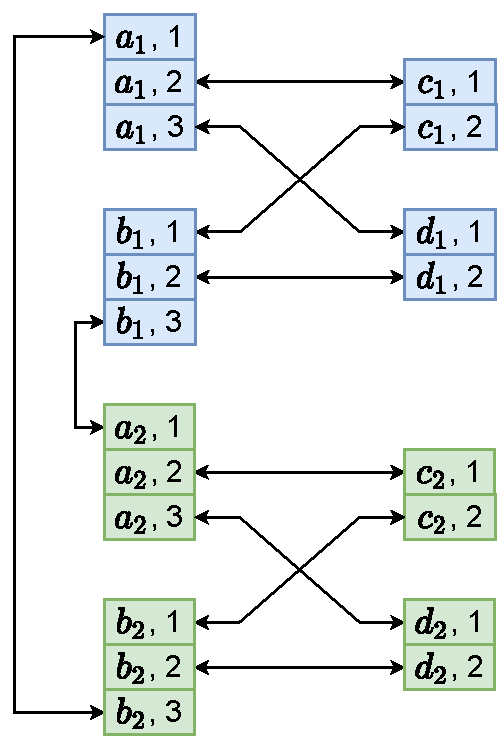
\includegraphics[scale=0.55]{diagrams/covering_map_1.pdf}
  }
  \hfill
  \subcaptionbox{
    A PN network N'.
    \label{fig:covering_map1:b}
  }%
    [.5\linewidth] {
    \centering
    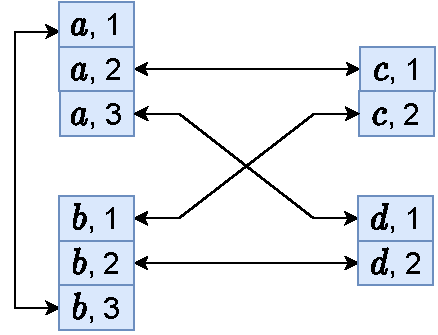
\includegraphics[scale=0.55]{diagrams/covering_map_2.pdf}
  }
  \caption{There is a covering map $\phi$ from $N$ to $N'$ that maps each $x_i$ to $x$ for all $x\in \{a, b, c, d\}$ and for all $i \in \{1, 2\}$.
  }
  \label{fig:covering_map1}
\end{figure}

\begin{figure}[H]
  \subcaptionbox{
    A PN network N.
    \label{fig:covering_map2:a}
  }%
    [.5\linewidth] {
    \centering
    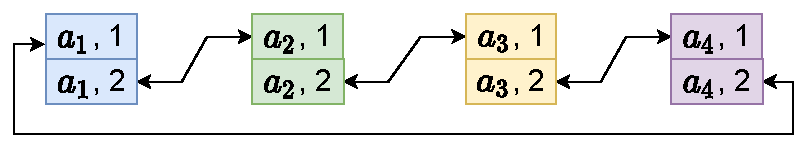
\includegraphics[scale=0.55]{diagrams/covering_map_3.pdf}
  }
  \hfill
  \subcaptionbox{
    A PN network N'.
    \label{fig:covering_map2:b}
  }%
    [.5\linewidth] {
    \centering
    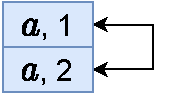
\includegraphics[scale=0.55]{diagrams/covering_map_4.pdf}
  }
  \caption{There is a covering map $\phi$ from $N$ to $N'$ that maps each $a_i$ to $a$ for all $i \in \{1, 2, 3, 4\}$.
  }
  \label{fig:covering_map2}
\end{figure}

There are two examples of covering maps on Figure \ref{fig:covering_map1} and \ref{fig:covering_map2}.
In these examples we can see that the sizes of covering networks are integer multiplications of the sizes of original networks.
This actually
\footnote{\todo{Do I need to show this?}}
applies to every covering map, i.e. if we have a covering map $\phi\colon V \rightarrow V'$, then $|V| = k|V'|$ for some $k \in \mathbb{N}_{>0}$ \cite{DBLP:journals/dm/GrossT77}.
We often call covering networks as \emph{lifts}.
A \emph{$k$-lift} is a lift where the covering network $N$ is $k$ times the size of $N'$.




\begin{figure}[H]
  \subcaptionbox{
    A PN network $N_0$ with loops.
    \label{fig:covering_map3:a}
  }%
    [.30\linewidth] {
    \centering
    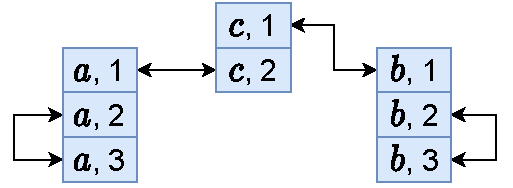
\includegraphics[scale=0.50]{diagrams/covering_map_5a.pdf}
  }
  \hfill
  \subcaptionbox{
    A PN network $N_1$ with multiple connections.
    \label{fig:covering_map3:b}
  }%
    [.30\linewidth] {
    \centering
    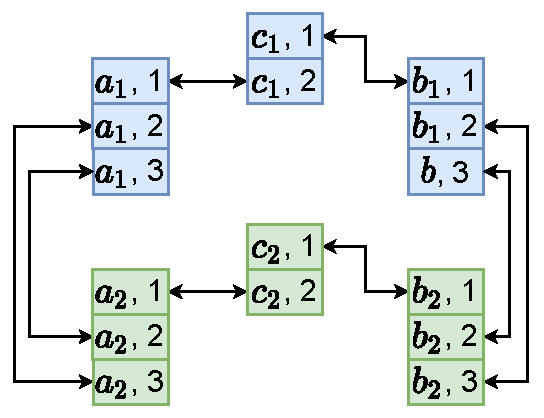
\includegraphics[scale=0.48]{diagrams/covering_map_5b.pdf}
  }
  \hfill
  \subcaptionbox{
    A simple PN network $N_2$.
    \label{fig:covering_map3:c}
  }%
    [.30\linewidth] {
    \centering
    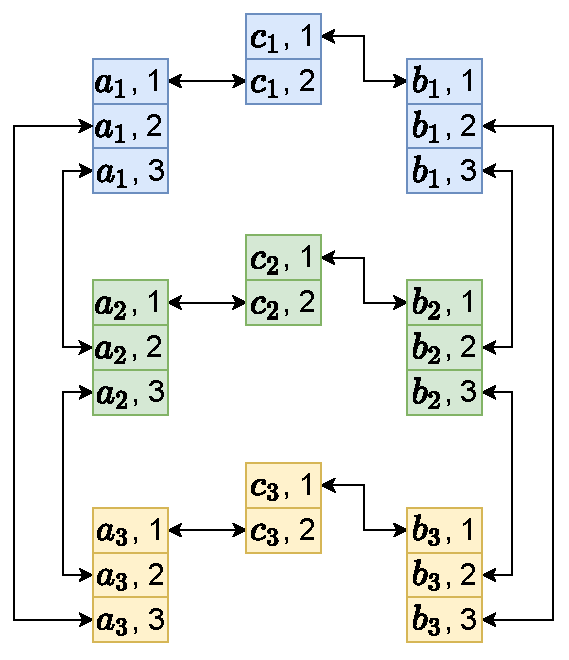
\includegraphics[scale=0.46]{diagrams/covering_map_5c.pdf}
  }
  \caption{
    There is a covering map $\phi_0$ from $N_1$ to $N_0$ that maps each $x_i$ to $x$ for all $x \in \{a, b, c\}$ and for all $i \in \{1, 2\}$.
    Similarly there is a covering map $\phi_1$ from $N_2$ to $N_0$ that maps each $x_i$ to $x$ for all $x \in \{a, b, c\}$ and for all $i \in \{1, 2, 3\}$.
  }
  \label{fig:covering_map3}
\end{figure}

In the Figure \ref{fig:covering_map3} we can see that the network $N_1$ is a 2-lift of the network $N_0$ and the network $N_2$ is a 3-lift of the network $N_0$.
The network $N_0$ has 2 loops, $p(p((a, 2))) = p((a, 3)) = (a, 2)$ and $p(p((b, 2))) = p((b, 3)) = (b, 2)$.



%\todo{explain lift}
%\begin{figure}[H]
%  \centering
%  \includegraphics[]{example-image-duck}
%  \caption{Show lift from N' to N}
%  \label{fig:duck2}
%\end{figure}
%%%This implies that the graphs $H$ and $G$ are indistinguishable from a PN algorithm's perspective.
%%%\cite{DBLP:conf/stoc/Angluin80}

% Let $H=(V', E')$ and $G=(V, E)$ be some graphs in the graph family $\mathcal{F}$.
% A covering map is a function $\Phi: V' \rightarrow V$ that maps the vertices $v' \in V'$ to vertices $v \in V$ in such a way that if

%The function that maps $H$ to $G$ is called a \emph{covering map}.

This symmetricity implies that each node ends up in an identical output state with its symmetrical equivalent given that the input problem $\Pi$ does not break the symmetry.
% In this section we are discussing about a graph theoretic method that can show

continue...........

\subsection{LOCAL model} \label{sec:local_model}
The LOCAL model is another message passing model that is used in the field of distributed computation.
It inherits from the PN model, hence most of the definition is already done in Section \ref{sec:formalized_pn_model}.
The difference is that the graph problem $\Pi'$, given as an input, is always predetermined.
A solution to problem $\Pi'$ is a node labeling $\operatorname{id}\colon V \rightarrow \{1,2,\dotsc,|V|\}$, where each node has a unique label \cite{DBLP:conf/focs/Linial87}.
Sometimes the node labeling is defined $\operatorname{id}\colon V \rightarrow \{1,2,\dotsc,|V|^c\}$, where $c$ is a positive constant greater than 1 \cite{HirvonenSuomelaDistAlg2020}, but in this work we assume $c=1$.
If a distributed algorithm $A$ solves a problem $\Pi$ on a graph family $\mathcal{F}$ given $\Pi'$, we say that $A$ solves $\Pi$ on graph family $\mathcal{F}$ in the LOCAL model \cite{HirvonenSuomelaDistAlg2020}.

Earlier in Section \ref{def:covering_map} we discussed about the limitation in a deterministic PN model that comes from symmetry.
In the LOCAL model, an algorithm can utilize these identifiers to break the symmetry and avoid the limitation of the PN model.

A well-known property of the LOCAL model is the ability to compute \emph{every} function of a graph $G$ in time $\mathcal{O}(\operatorname{diameter}(G))$.
This amount of time is enough for any node in $G$ to gather complete information of both the graph and the unique labels from function $\operatorname{id}$, because a message can travel from a node to any other node at most in $\operatorname{diameter}(G)$ time.
With the complete information of everything, each node can compute the whole solution and output its own part of the solution.
Because of this, researchers are usually interested in complexity classes below the $\mathcal{O}(\operatorname{diameter}(G))$.

\todo{Discuss more about LOCAL? }

\subsection{Locally checkable labeling problems} \label{sec:lcl_problems}
In this section we define \emph{Locally checkable labeling (LCL)} problems generally.
This section is intended as an introduction for the Section \ref{sec:lcl_problems:biregular} where we introduce an alternative definition of LCL problems that we will be using in this work.
Briefly, LCL problems are a family of graph problems where a global solution (node labeling) can be verified locally by the individual nodes.


%TODO move this commented paragraph to somewhere where we talk about locality and complexity.
%LCL problems were first introduced in the paper \cite{DBLP:journals/siamcomp/NaorS95} by Moni Naor and Larry Stockmeyer in 1995.
%The paper laid the groundwork for further researches of the locality of distributed graph problems.
%\emph{Locality} is the maximum distance each node has to gather information from, in order to choose an output \cite{DBLP:journals/sigact/Suomela20}.
%Instead of discussing about locality, we can equally talk about round complexity of message passing algorithms \cite{DBLP:journals/sigact/Suomela20}.
%\todo{talk something about the constant radius and every t-time problem basically has to form the output based on the t-radius neighourhood (the information about the t-radius network the nodes have gathered) }.

\newcommand{\Sigmain}{\Sigma_{\text{in}}}
\newcommand{\Sigmaout}{\Sigma_{\text{out}}}


Now we define LCL problems using the formalism from the paper \cite{DBLP:journals/siamcomp/NaorS95} and we also use the formalism from a more recent paper \cite{DBLP:journals/corr/abs-2105-05574}.
An LCL problem $\Pi$ consists of:
\begin{itemize}
  \item a positive integer $r$, which is called the \emph{radius} of $\Pi$,
  \item a finite set of \emph{input labels} $\Sigmain$,
  \item a finite set of \emph{output labels} $\Sigmaout$ and
  \item a finite set of \emph{locally consistent labelings} $C$, where:
  \begin{itemize}
    \item the elements are pairs $(H=(V^H, E^H), s)$,
    \item $H$ is a graph, node $s$ is in $V^H$, and the distance from the node $s$ to any other node in $V^H$ is at most $r$,
    \item every pair $(v, e) \in (V^H \times E^H)$ is labeled with a pair from $\Sigmain \times \Sigmaout$.
  \end{itemize}
\end{itemize}
Given a graph $G = (V, E)$ and a node labeling $f: V \rightarrow \Sigmain \times \Sigmaout$, the node labeling $f$ is a solution to an LCL problem $\Pi$ if for every node $v \in V$, the $r$-radius ball $B_G(v, r)$ is isomorphic to some labeled graph in $C$ \cite{DBLP:journals/corr/abs-2105-05574}.

Several common graph problems are in the LCL family.
For example the problems introduced in Section \ref{sec:dist_graph_probl} are LCL problems.
We now define these problems using the LCL notation.
The input is unnecessary for each of these problems,
therefore we set the input labels $\Sigmain = \{1\}$ for each problem.
Each problem has radius 1.
Listing the locally consistent labelings of each problem would result in substantially large sets of graphs, hence we give only a brief description of the elements.
\begin{description}
  \item[$k$-coloring] The set of output labels $\Sigmaout$ contains all $k$ colors, e.g. $1, 2, \dotsc, k$.
  The set $C$ contains all the possible 1-ball graphs of a given graph family with all possible combinations of vertex colorings with $k$-colors.
  \item[Maximal independent set]
  The set of output labels $\Sigmaout$ contains labels 0 and 1.
  The set $C$ contains all the possible 1-ball graphs of a given graph family with all possible combinations of output labels such that if and only if the node $s$ (the center node) is $1$, then all adjacent nodes are labelled with $0$.
  Label 0 denotes that the vertex is not in the maximal independent set, and label 1 denotes that it is in the set.
  \item[Minimal vertex cover]
  The set of output labels $\Sigmaout$ contains labels 0 and 1.
  The set $C$ contains all the possible 1-ball graphs of a given graph family with all possible combinations of output labels such that if and only if the node $s$ (the center node) is $0$, then all adjacent nodes are labelled with $1$.
  Label 0 denotes that the vertex is not in the minimal vertex cover, and label 1 denotes that it is in the set.
  \footnote{This problem is a complement of the maximal independent set.}
\end{description}

It is clear that defining the whole set $C$ explicitly in this formalism would be a substantial amount of work, at least when radius $r$ is high.
Therefore we depend on another formalism of LCL problems that provides a more compact representation of the problems.
\todo{Aren't there more reasons?}


\subsection{LCL problems in biregular graphs} \label{sec:lcl_problems:biregular}
In this section, we will introduce an alternative formalism of LCL problems used in this work, that originates from paper \cite{DBLP:conf/podc/Brandt19}, and recently it has been seen in the papers including \cite{DBLP:conf/podc/Olivetti20} and \cite{DBLP:journals/sigact/Suomela20}.
We will be referring to these papers in the following definitions.

In the formalism, LCL problems are generally defined for \emph{infinite $\Delta$-regular $\delta$-uniform hypertrees} \cite{DBLP:conf/podc/Olivetti20}.
Hypertrees are hypergraphs with tree structure.
Hypergraph is a generalization of graphs.
The concept of hypergraphs might first seem difficult to understand.
It simply means that an edge is called as a hyperedge, and it can connect \emph{any} number of nodes.
To be $\delta$-uniform means that the hyperedges connect to exactly $\delta$ nodes.
Note that if we fix $\delta=2$, then the problems are defined for infinite $\Delta$-regular trees \cite{DBLP:conf/podc/Olivetti20}.

An LCL problem $\Pi$ is a tuple $(\Sigma, A, P)$, where $\Sigma$ is a finite set of labels, and $A$ and $P$ are finite sets containing all allowed \emph{label configurations} of nodes and hyperedges, respectively.
A label configuration is a multiset containing labels from the set $\Sigma$.
The label configurations in $A$ have a length of $\Delta$ and the label configurations in $P$ have a length of $\delta$ \cite{DBLP:journals/sigact/Suomela20}.

The task of each node is to label each of its incident hyperedge with a label from $\Sigma$ \cite{DBLP:journals/sigact/Suomela20}.
Each node will label $\Delta$ incident hyperedges, thus each hyperedge will be labeled with $\delta$ labels.
The labels given by a node to its incident hyperedges form a label configuration.
Similarly the labels given to a hyperedge form a label configuration.
Label configurations of a node have a length of $\Delta$ and label configurations of a hyperedge have a length of $\delta$.
We require from a solution that:
\begin{enumerate}
  \item every label configuration of a node is contained in $A$, and
  \item every label configuration of a hyperedge is contained in $P$.
\end{enumerate}

Alternatively to $\Delta$-regular $\delta$-uniform hypertrees, we can think of the hyperedges as a separate nodes \cite{DBLP:conf/podc/Olivetti20}.
This way the problems are defined for infinite $(\Delta, \delta)$-biregular trees.
We say that the original nodes of the graph are called \emph{active nodes}, and the newly introduced nodes, formerly hyperedges, are called \emph{passive nodes}.
%This naming convention can be seen in the sets $A$ and $P$.
%In  which can be called as the sets of active constraints and passive constraints, respectively.
In this setting the passive nodes do not output anything.
Only the active nodes output their labels.

We showed some examples of LCL problems in Section \ref{sec:lcl_problems}.
Now we show some of the problems in the alternative formalism.

The sets $\Sigma, A$ and $P$ of $k$-coloring in infinite (3,2)-biregular graphs are defined as:
\begin{align*}
  \Sigma &= \{1, 2, \dotsc, k\}, \\
  A &= \{\{1,1,1\},\{2,2,2\},\dotsc,\{k,k,k\}\}, \\
  P &= \{\{a, b\}\mid a,b,\in \Sigma \text{ and } a \neq b\}.
\end{align*}
An active node has a color between 1 and $k$.
All label configurations of active nodes correspond to a single color.
The label configurations of passive nodes ensure that the neighbours of an passive node do not share a color.
For an example, see Figure~\ref{fig:biregular_graph1}.

\begin{figure}[H]
  \subcaptionbox{
    An infinite $(3,2)$-biregular tree.
    Orange nodes are active nodes, and smaller blue nodes are passive nodes.
    The labels seen in the graph are part of a solution to maximal independent set problem.
    \label{fig:biregular_graph1:a}
  }%
    [0.60\linewidth] {
    \centering
    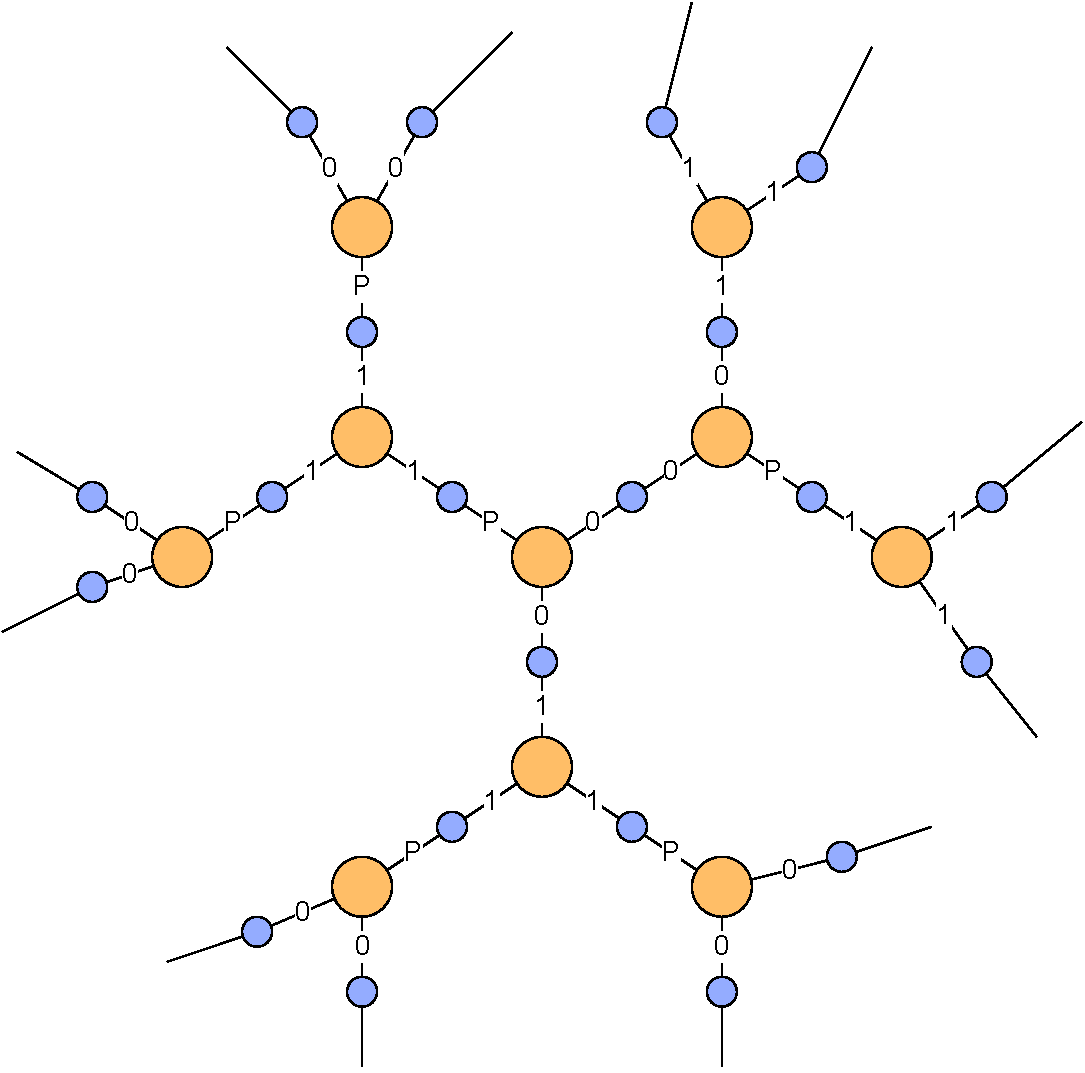
\includegraphics[scale=0.45]{diagrams/biregular_graph_LCL_MIS.pdf}
  }
  \hfill
  \subcaptionbox{
    Same graph as in \ref{fig:biregular_graph1:a}, but the passive nodes are seen as 2-uniform hyperedges, or just as edges, and the nodes are now colored.
    %The nodes with label 1 map to nodes in \ref{fig:biregular_graph2:a} with node label $\{1,1,1\}$ and nodes with label 0 map to nodes in \ref{fig:biregular_graph2:a} with node label $\{P,0,0\}$.
    \label{fig:biregular_graph1:b}
  }%
    [.35\linewidth] {
    \centering
    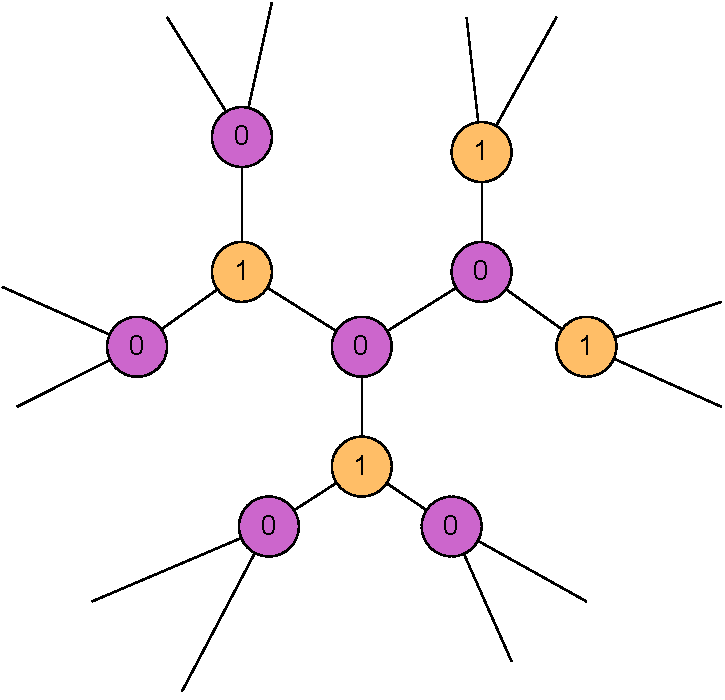
\includegraphics[scale=0.40]{diagrams/biregular_graph_LCL_MIS2.pdf}
  }
  \caption{
    3-coloring in infinite $(3,2)$-biregular tree.
  }
  \label{fig:biregular_graph1}
\end{figure}

The sets $\Sigma, A$ and $P$ of maximal independent set in infinite (3,2)-biregular graphs are defined \cite{HirvonenSuomelaDistAlg2020} as :
\begin{align*}
  \Sigma &= \mathrm{\{I,O,P\}}, \\
  A &= \mathrm{\{\{I,I,I\},\{P,O,O\}\}}, \\
  P &= \mathrm{\{\{I,P\},\{I,O\},\{O,O\}\}}.
\end{align*}
An active node with label configuration $\mathrm{\{I,I,I\}}$ is considered to be in the maximal independent set and label configuration $\mathrm{\{P,O,O\}}$ means that the node is not in the set.
The label configurations of passive nodes ensure that the output of active nodes is an independent set, and the label $\mathrm{P}$ ensures that the set is maximal \cite{HirvonenSuomelaDistAlg2020}.
For an example, see Figure~\ref{fig:biregular_graph2}.

\begin{figure}[H]
  \subcaptionbox{
    An infinite $(3,2)$-biregular tree.
    Orange nodes are active nodes, and smaller blue nodes are passive nodes.
    The labels seen in the graph are part of a solution to maximal independent set problem.
    \label{fig:biregular_graph2:a}
  }%
    [0.60\linewidth] {
    \centering
    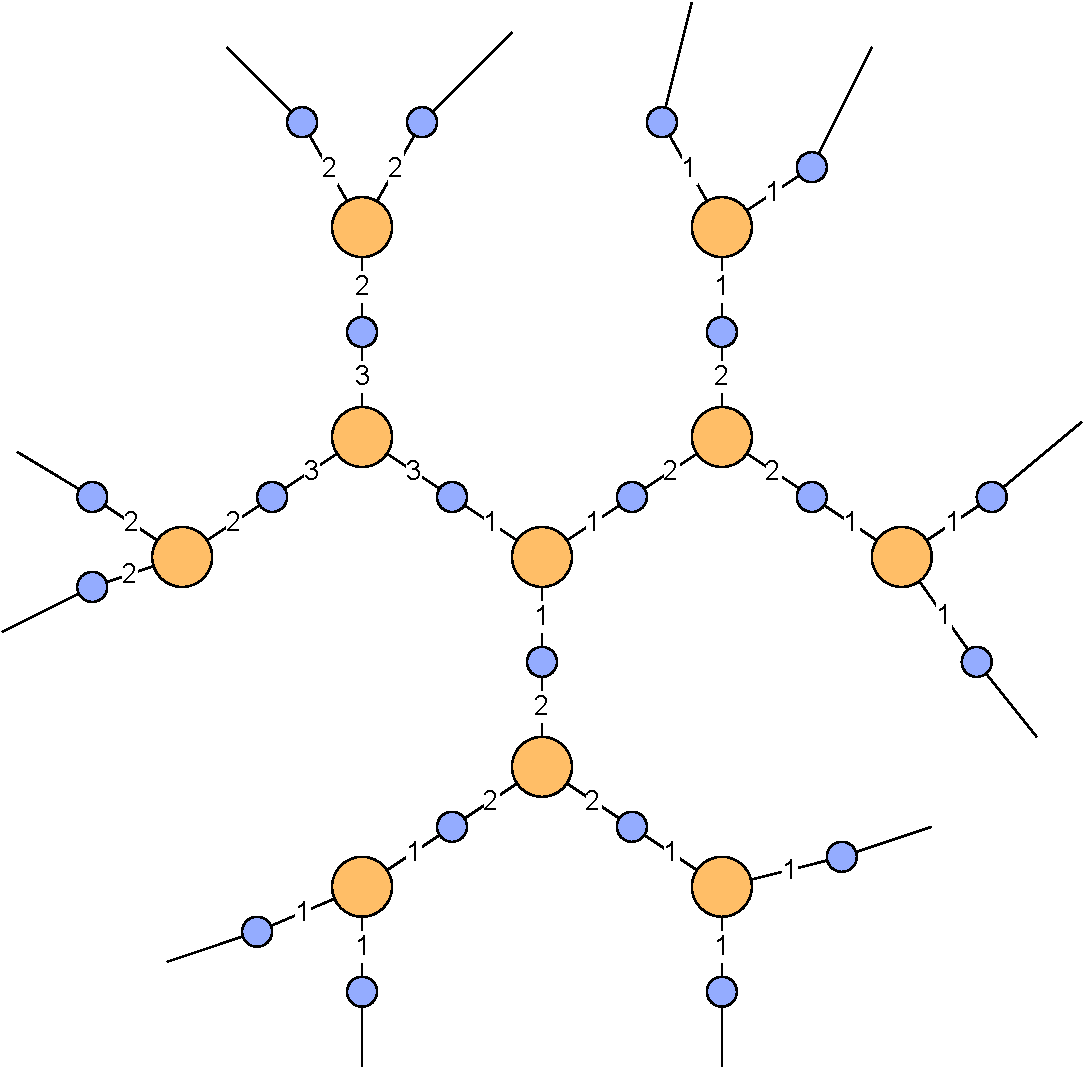
\includegraphics[scale=0.45]{diagrams/biregular_graph_LCL_3Coloring.pdf}
  }
  \hfill
  \subcaptionbox{
    A visualization of the coloring in graph \ref{fig:biregular_graph2:a}.
    The graphs are identical, but the passive nodes are seen as 2-uniform hyperedges, or just as edges.
    \label{fig:biregular_graph2:b}
  }%
    [.35\linewidth] {
    \centering
    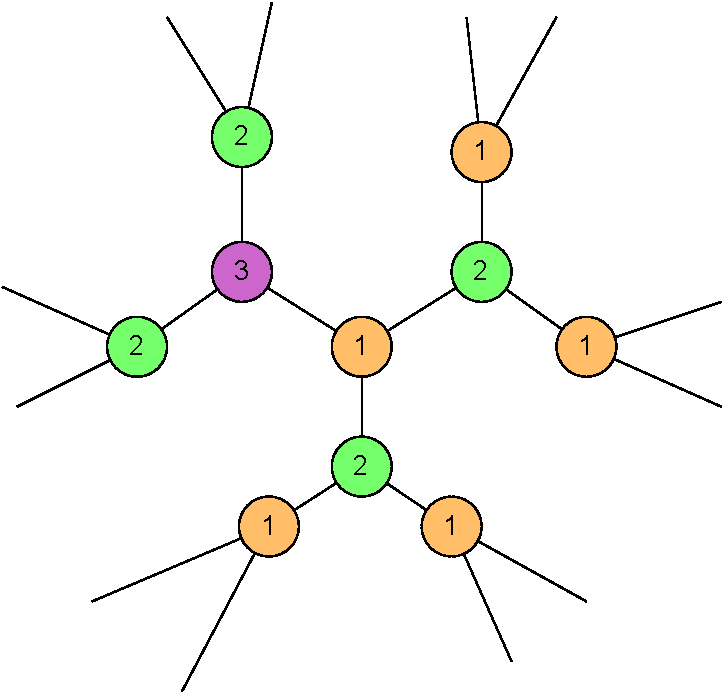
\includegraphics[scale=0.40]{diagrams/biregular_graph_LCL_3Coloring_2.pdf}
  }
  \caption{
    Maximal independent set in infinite $(3,2)$-biregular tree.
  }
  \label{fig:biregular_graph2}
\end{figure}

\todo{Address the fact that this definition is for infinite hypertrees. Can we use it with finite graphs?}


\subsection{Boolean satisfiability problem}
\todo{Explain
\begin{itemize}
  \item SAT problems, %TODO
  \item DIMACS CNF, %TODO
  \item SAT solvers, %TODO
\end{itemize}
I am not sure if these are even needed.
I could just assume that the reader knows the basics.
}


\clearpage

